%% LaTeX Beamer presentation template (requires beamer package)
%% see http://bitbucket.org/rivanvx/beamer/wiki/Home
%% idea contributed by H. Turgut Uyar
%% template based on a template by Till Tantau
%% this template is still evolving - it might differ in future releases!

\documentclass{beamer}

\mode<presentation>
{
\usetheme{Warsaw}

\setbeamercovered{transparent}
}

%%%%%%%%%%%%%%
%% PACKAGES %%
%%%%%%%%%%%%%%

\usepackage{fontspec}
%     \usepackage{libertineotf}

% \usepackage{setspace} % Change spacing between lines
% %  	{\setstretch{5.0} text}

\usepackage{xcolor,graphicx}

\usepackage{sty/onimage}
	\usetikzlibrary{positioning}


\usepackage{hyphenat} % Can allow wordbreaks anywhere using -> \hyphenation{none}

% \usepackage[english]{babel}
% \usepackage[latin1]{inputenc}
% 
% % font definitions, try \usepackage{ae} instead of the following
% % three lines if you don't like this look
% \usepackage{mathptmx}
% \usepackage[scaled=.90]{helvet}
% \usepackage{courier}

\usepackage{ifluatex,ifxetex}

% \usepackage[T1]{fontenc}

\usepackage{xargs} % Allows for more than 1 optional argument in a command
\usepackage{xifthen}% provides \isempty test

%%%%%%%%%%%%%%
%%  COLORS  %%
%%%%%%%%%%%%%%
\definecolor{TIBG}{rgb}{0.75,0.8235,0.75}% TI background color

%%%%%%%%%%%%%%
%% COMMANDS %%
%%%%%%%%%%%%%%

%% FIGURES %%

% http://tex.stackexchange.com/questions/53998/beamer-how-text-wrapping-around-a-graphic-right-aligned
\newcommand{\lenitem}[2][.8\linewidth]{\parbox[t]{#1}{\strut #2\strut}} % Wrap text in a fixed-size parbox environment.




    
    
    
%% TI Calculator top-right corner %%

\def\ticalcfigCircleButtonsize{0.021\textheight}
\def\ticalcfigCircleNumButtonsize{0.0255\textheight}
\def\ticalcfigCircleEnterButtonsize{0.028\textheight}
\def\ticalcfigCircleBigButtonsize{0.05\textheight}
% #1 (optional) = radius of circle
% #2 (obligatory) = x of circle center
% #3 (obligatory) = y of circle center
\newcommand{\ticalcfigCircle}[3][\ticalcfigCircleButtonsize]{\draw [green, line width=1pt] (#2,#3) circle [radius=#1];}
\def\ticalcfigCircleColOne{0.130}
\def\ticalcfigCircleColTwo{0.314}
\def\ticalcfigCircleColThree{0.502}
\def\ticalcfigCircleColFour{0.690}
\def\ticalcfigCircleColFive{0.878}
\def\ticalcfigCircleAlpha{\ticalcfigCircle{\ticalcfigCircleColOne}{0.739}}
\def\ticalcfigCircleSecond{\ticalcfigCircle{\ticalcfigCircleColOne}{0.816}}
\def\ticalcfigCircleEnter{\ticalcfigCircle[\ticalcfigCircleEnterButtonsize]{0.868}{0.128}}
\def\ticalcfigCircleLeft{\ticalcfigCircle{0.695}{0.79}}
\def\ticalcfigCircleDown{\ticalcfigCircle{0.815}{0.733}}
\def\ticalcfigCircleRight{\ticalcfigCircle{0.916}{0.79}} % This circle is shifted to the left ... Otherwise it would fall out of the image, which would shift the entire image to the left on the slide. TODO: Better alternative?
\def\ticalcfigCircleUp{\ticalcfigCircle{0.815}{0.85}}
\def\ticalcfigCircleArrowkeys{\ticalcfigCircle[\ticalcfigCircleBigButtonsize]{0.815}{0.79}}


% #1 (optional) = figure height
% #2 (obligatory) = body of tikzonimage environment. Use \ticalcfigCircle zero or more times.
% #3 (optional) = activate grid for debugging? Empty = no, Something = yes.
\newcommandx{\ticalcfig}[3][1=0.5\textheight, 3=]{
\begin{tikzpicture}[overlay,remember picture]
	\node[] (TR) at (current page.north east){ };
	\node [anchor=north east,xshift=0.05cm,yshift=-1.4cm] at (TR)
	{\ifthenelse{\isempty{#3}}{% if #3 is empty
		\begin{tikzonimage}[height=#1]{TI84_buttons.png}
			#2
		\end{tikzonimage}
	}{% if #3 is not empty
		\begin{tikzonimage}[height=#1]{TI84_buttons.png}[tsx/show help lines]
			#2
		\end{tikzonimage}
	}};
\end{tikzpicture}
}



%% FONT %%

% This heavily uses the 'graphicx' package.
% Define all custom characters (like unequals) and characters not accessible by the keyboard (like sigma).
\def\tidefinechars{\catcode`\;12 \catcode`\:12 \catcode`\!12 \catcode`\?12 \catcode`\^^M12 \catcode`\ 12%
	\def\>{-\llap{\lower0.131em\hbox{`}\llap{\lower0.374em\hbox{\reflectbox{`}}\kern0.125em }\kern-0.122em}\kern0.18em}% Sto ->
	\def\!{=\llap{/}}% Unequal
	\def\sqrt{\XeTeXglyph95\llap{\lower0.5em\hbox{`}\kern0em}\llap{\lower-0.377em\hbox{\scalebox{0.5}[1]{-}}\kern-0.170em}}% Sqrt
	\def\arrowdown{\kern-0.5em\lower-0.88em\hbox{\scalebox{0.75}[1]{\scalebox{1.2}{\rotatebox{-90}{\>\kern-0.18em}}}}\kern0.2em}% Arrow pointing downwards (used in menus to indicate that there is something below)
	\def\arrowup{\kern-0.01em\lower-0.86em\hbox{\reflectbox{\rotatebox{180}{\arrowdown}}}}% Arrow pointing downwards (used in menus to indicate that there is something below)
	\def\:{:\kern0.2em}% Increase kerning behind the colon (:)
	\def\+{\kern0.13em}% Increase spacing between previous and next character: 'kerning'.
	\def\sq{{\XeTeXglyph101}}% Square (power 2)
	\def\cube{{\XeTeXglyph102}}% Cube (power 3)
	\def\deg{{\XeTeXglyph100}}% degree symbol
	\def\Delta{{\XeTeXglyph153}}% Delta
	\def\theta{{\XeTeXglyph154}}% theta
	\def\Sigma{{\XeTeXglyph155}}% Sigma
	\def\Omega{{\XeTeXglyph156}}% Omega
	\def\alpha{{\XeTeXglyph157}}% alpha
	\def\beta{{\XeTeXglyph158}}% beta
	\def\gamma{{\XeTeXglyph159}}% gamma
	\def\delta{{\XeTeXglyph160}}% delta
	\def\eps{{\XeTeXglyph161}}% epsilon
	\def\ci{{\XeTeXglyph162}}% complex i / iota
	\def\iota{{\XeTeXglyph162}}% complex i / iota
	\def\lambda{{\XeTeXglyph163}}% lambda
	\def\mu{{\XeTeXglyph164}}% mu
	\def\pi{{\XeTeXglyph165}}% pi
	\def\rho{{\XeTeXglyph166}}% rho
	\def\sigma{{\XeTeXglyph167}}% sigma
	\def\tau{{\XeTeXglyph168}}% tau
	\def\phi{{\XeTeXglyph169}}% phi
	\def\xi{{\XeTeXglyph170}}% xi
	\def\ldots{{\XeTeXglyph171}}% ldots
	\def\percent{{\XeTeXglyph8}}% %
	\def\dollar{{\XeTeXglyph7}}% $
	\def\and{{\XeTeXglyph9}}% &
	\def\qt{{\XeTeXglyph5}}% quote "
	\def\quote{{\XeTeXglyph5}}% quote "
	\def\function{{\XeTeXglyph0}}% f with black-white inverted
	\def\~{{\XeTeXglyph97}}% ~
	\def\^{{\XeTeXglyph65}}% ^
	\def\#{{\XeTeXglyph6}}% #
 	\def\_##1{\scalebox{0.6}{##1}\scalebox{0.4}{ }}% subscript, e.g. to create Y1 with a small 1.
%  	\setlength{\columnsep}{15pt}
 	\def\,{\hspace{1ex}}% Custom spacebar size, useful for strings.
 	\def\select##1{\fboxrule0pt\fboxsep0.2pt% Select the text
		\fcolorbox{black}{green!0!black!100}{%
			\color{TIBG}{##1}%
		}}% Colors the background as the text and text as the background: 'selection box'.
 	\def\selectitem##1{\fboxrule0pt\fboxsep0pt% Like \select, but special for selecting menu items. Input: number
		\fcolorbox{black}{green!0!black!100}{%
			\color{TIBG}{##1}\kern-0.15em%
		}\kern0.15em}% Colors the background as the text and text as the background: 'selection box'.
}%

\newfontfamily\tifont[Path=font/]{TI83_font.ttf}
\newcommand{\tifonttxt}[1]{{\tifont\tidefinechars\scriptsize#1}}
\newcommand{\tifontbigtxt}[1]{{\tifont\tidefinechars\normalsize#1}}

\newfontfamily\TIbutton[Path=font/]{TI83_button.ttf}
\DeclareTextFontCommand{\TI}{\TIbutton}
\ifluatex
 \def\tibutton#1{\TI{\directlua{fonts.otf.char("#1")}}}
 \newcommand{\tibuttonnum}[1]{\TI{#1}}% Does not work! I use XeTeX, I don't know about Lua.
\fi
\ifxetex
 \def\tibutton#1{\TI{\XeTeXglyph\the\XeTeXglyphindex"#1"}}
%  \def\tibuttonnum#1{\TI{\XeTeXglyph#1}}
 \newcommand{\tibuttonnum}[1]{\TI{\XeTeXglyph#1}}
\fi

\newsavebox{\selvestebox}
\newenvironment{ticalc}[1][3.25cm]{%[1=\dimexpr\columnwidth-2\fboxsep\relax]{% %TODO: Default does not work.
	% Define environment
	\tifont\tidefinechars\scriptsize%\addfontfeature{LetterSpace=10.0}%
	\begin{lrbox}{\selvestebox}%
	\begin{minipage}{#1}
	\begin{flushleft}
}{
	\end{flushleft}
	\end{minipage}\end{lrbox}%
	\begin{centering}
	\fboxrule1pt\fboxsep2pt
	\fcolorbox{black}{green!30!black!25}{
		\hyphenation{none}\usebox{\selvestebox}
	}
	\end{centering}
}

\newcommand{\inlineticalc}[1]{{% Inline TI calculator within a box. Does not permit enters (//)!
	% Define environment
	\tifont\tidefinechars\scriptsize%\addfontfeature{LetterSpace=0.0}
	\fboxrule0.8pt\fboxsep1pt
	\fcolorbox{black}{green!30!black!25}{
		#1
	}
}}





    
%%%%%%%%%%%%%%%%%%
%% TI Shortcuts %%
%%%%%%%%%%%%%%%%%%

% Test/Logic
\newcommand{\tiGT}			{\tibuttonnum{20}}
\newcommand{\tiMGT}			{\tibuttonnum{21}}
\newcommand{\tiGTO}			{\tibuttonnum{22}}

% Menu buttons
\newcommand{\tiQUIT}		{\tibuttonnum{24}}
\newcommand{\tiINS}			{\tibuttonnum{25}}
\newcommand{\tiALOCK}		{\tibuttonnum{26}}
\newcommand{\tiLINK}		{\tibuttonnum{27}}
\newcommand{\tiLIST}		{\tibuttonnum{28}}
\newcommand{\tiTEST}		{\tibuttonnum{29}}
\newcommand{\tiANGLE}		{\tibuttonnum{30}}
\newcommand{\tiDRAW}		{\tibuttonnum{31}}
\newcommand{\tiDISTR}		{\tibuttonnum{32}}
\newcommand{\tiMATRIX}		{\tibuttonnum{33}}
\newcommand{\tiMATRX}		{\tibuttonnum{52}}
\newcommand{\tiMATRXBut}	{\tibuttonnum{112}}
\newcommand{\tiMEM}			{\tibuttonnum{47}} % Memory
\newcommand{\tiCATALOG}		{\tibuttonnum{49}} % Catalog
\newcommand{\tiFINANCE}		{\tibuttonnum{56}} % Finance
\newcommand{\tiMODE}		{\tibuttonnum{93}}
\newcommand{\tiSTAT}		{\tibuttonnum{103}}
\newcommand{\tiAPPS}		{\tibuttonnum{110}}
\newcommand{\tiMATH}		{\tibuttonnum{111}}
\newcommand{\tiPRGM}		{\tibuttonnum{113}}
\newcommand{\tiVARS}		{\tibuttonnum{114}}
\newcommand{\tiYVARS}		{\tibuttonnum{212}} % Y-VARS

% Formula buttons (sqrt, etc.)
\newcommand{\tiSIN}			{\tibuttonnum{122}}
\newcommand{\tiCOS}			{\tibuttonnum{123}}
\newcommand{\tiTAN}			{\tibuttonnum{124}}
\newcommand{\tiASIN}		{\tibuttonnum{34}}
\newcommand{\tiACOS}		{\tibuttonnum{35}}
\newcommand{\tiATAN}		{\tibuttonnum{36}}
\newcommand{\tipi}			{\tibuttonnum{37}} % Small pi with [] around it
\newcommand{\tiPI}			{\tibuttonnum{51}} % Capital PI (Product sign)
\newcommand{\tiSIGMA}		{\tibuttonnum{54}} % Capital sigma (Sum sign)

\newcommand{\tiLCB}			{\tibuttonnum{40}} % Left curly bracket  {
\newcommand{\tiLPAREN}		{\tibuttonnum{40}} % Left Parenthesis (=LCB)
\newcommand{\tiRCB}			{\tibuttonnum{41}} % Right curly bracket }
\newcommand{\tiRPAREN}		{\tibuttonnum{41}} % Right Parenthesis (=RCB)
\newcommand{\tiLSB}			{\tibuttonnum{43}} % Left square bracket:  [
\newcommand{\tiRSB}			{\tibuttonnum{44}} % Right square bracket: ]
\newcommand{\tiLRB}			{\tibuttonnum{133}} % Left round bracket: (
\newcommand{\tiRRB}			{\tibuttonnum{134}} % Right round bracket: )

\newcommand{\tiEE}			{\tibuttonnum{39}} % 1E2 = 100
\newcommand{\tiTENPOWER}	{\tibuttonnum{42}} % 10^x
\newcommand{\tiEPOWER}		{\tibuttonnum{45}} % e^x
\newcommand{\tiXInv}		{\tibuttonnum{121}} % x^-1 -> Inverse of x
\newcommand{\tiLOG}			{\tibuttonnum{141}} % log
\newcommand{\tiLN}			{\tibuttonnum{151}} % ln

\newcommand{\tiNeg}			{\tibuttonnum{174}} % (-) -> negative number
\newcommand{\tiDot}			{\tibuttonnum{173}} % .
\newcommand{\tii}			{\tibuttonnum{57}} % Imaginary number (button)
\newcommand{\tiiScreen}		{\tibuttonnum{185}} % Imaginary number (on-screen)

\newcommand{\tiTimes}		{\tibuttonnum{145}} % a x b -> product
\newcommand{\tiProduct}		{\tibuttonnum{145}} % a x b -> product
\newcommand{\tiMultiply}	{\tibuttonnum{145}} % a x b -> product
\newcommand{\tiMinus}		{\tibuttonnum{155}} % a - b -> subtraction
\newcommand{\tiPlus}		{\tibuttonnum{165}} % a + b -> addition
\newcommand{\tiDivide}		{\tibuttonnum{135}} % a / b -> division
\newcommand{\tiDivision}	{\tibuttonnum{135}} % a / b -> division
\newcommand{\tiOver}		{\tibuttonnum{135}} % a / b -> division
\newcommand{\tiPower}		{\tibuttonnum{125}} % a ^ b -> power

% Numbers
\newcommand{\tiZero}		{\tibuttonnum{172}}
\newcommand{\tiOne}			{\tibuttonnum{162}}
\newcommand{\tiTwo}			{\tibuttonnum{163}}
\newcommand{\tiThree}		{\tibuttonnum{164}}
\newcommand{\tiFour}		{\tibuttonnum{152}}
\newcommand{\tiFive}		{\tibuttonnum{153}}
\newcommand{\tiSix}			{\tibuttonnum{154}}
\newcommand{\tiSeven}		{\tibuttonnum{142}}
\newcommand{\tiEight}		{\tibuttonnum{143}}
\newcommand{\tiNine}		{\tibuttonnum{144}}

% Other buttons
\newcommand{\tiRCL}			{\tibuttonnum{46}} % Recall variable
\newcommand{\tiOFF}			{\tibuttonnum{48}}
\newcommand{\tiON}			{\tibuttonnum{171}}
\newcommand{\tiONHALT}		{\tibuttonnum{147}} % ON/HALT
\newcommand{\tiANS}			{\tibuttonnum{61}}
\newcommand{\tiDEL}			{\tibuttonnum{94}}
\newcommand{\tiCLEAR}		{\tibuttonnum{115}}

\newcommand{\tiLeft}		{\tibuttonnum{95}}
\newcommand{\tiUp}			{\tibuttonnum{96}}
\newcommand{\tiRight}		{\tibuttonnum{97}}
\newcommand{\tiDown}		{\tibuttonnum{104}}

\newcommand{\tiSpace}		{\tibuttonnum{10}} % Visible spacebar
\newcommand{\tiSpaceButton}	{\tibuttonnum{50}} % Visible spacebar with [] around it

\newcommand{\tiSecond}		{\tibuttonnum{92}} % 2nd
\newcommand{\tiALPHA}		{\tibuttonnum{101}}

\newcommand{\tiENTER}		{\tibuttonnum{175}}
\newcommand{\tiENTRY}		{\tibuttonnum{62}}
\newcommand{\tiSOLVE}		{\tibuttonnum{63}}

\newcommand{\tiXTn}			{\tibuttonnum{102}} % X, T, Theta, n

\newcommand{\tiTRIGGER}		{\tibuttonnum{146}}

\newcommand{\tiSTO}			{\tibuttonnum{161}} % STO> button (store number into a var)

\newcommand{\tiCONT}		{\tibuttonnum{209}}

\newcommand{\tin}			{\tibuttonnum{213}} % small n (parameter of recursion)
\newcommand{\tiunmOne}		{\tibuttonnum{214}} % small u_n-1 (parameter of recursion)
\newcommand{\tivnmOne}		{\tibuttonnum{215}} % small v_n-1 (parameter of recursion)

% List
\newcommand{\tiLOne}		{\tibuttonnum{71}}
\newcommand{\tiLTwo}		{\tibuttonnum{72}}
\newcommand{\tiLThree}		{\tibuttonnum{73}}
\newcommand{\tiLFour}		{\tibuttonnum{74}}
\newcommand{\tiLFive}		{\tibuttonnum{75}}
\newcommand{\tiLSix}		{\tibuttonnum{76}}

% F buttons
\newcommand{\tiFOne}		{\tibuttonnum{65}}
\newcommand{\tiFTwo}		{\tibuttonnum{66}}
\newcommand{\tiFThree}		{\tibuttonnum{67}}
\newcommand{\tiFFour}		{\tibuttonnum{68}}
\newcommand{\tiFFive}		{\tibuttonnum{69}}

% Graphing
\newcommand{\tiYEquals}		{\tibuttonnum{82}} % Y=
\newcommand{\tiWINDOW}		{\tibuttonnum{83}}
\newcommand{\tiZOOM}		{\tibuttonnum{84}}
\newcommand{\tiTRACE}		{\tibuttonnum{85}}
\newcommand{\tiGRAPH}		{\tibuttonnum{86}}
\newcommand{\tiSTATPLOT}	{\tibuttonnum{15}}
\newcommand{\tiTBLSET}		{\tibuttonnum{16}}
\newcommand{\tiFORMAT}		{\tibuttonnum{17}}
\newcommand{\tiCALC}		{\tibuttonnum{18}}
\newcommand{\tiTABLE}		{\tibuttonnum{19}}

\newcommand{\tiBarGraph}	{\tibuttonnum{180}} % Icon for a bar graph
\newcommand{\tiLineGraph}	{\tibuttonnum{181}} % Icon for a line graph
\newcommand{\tiLinearGraph}	{\tibuttonnum{182}} % Linear line graph
\newcommand{\tiSpreadGraph}	{\tibuttonnum{183}} % Spread graph
\newcommand{\tiDoubleSpreadGraph}{\tibuttonnum{184}} % Spread graph with quadrants

\newcommand{\tiDotGraph}	{\tibuttonnum{5}} % Graph icon showing separate dots

\newcommand{\tiGraphIsLine}		{\tibuttonnum{201}} % Normal graph line
\newcommand{\tiGraphIsThick}	{\tibuttonnum{202}} % Thick line graph
\newcommand{\tiGraphIsFillUp}	{\tibuttonnum{203}} % Fill above the line
\newcommand{\tiGraphIsFillDown}	{\tibuttonnum{204}} % Fill beneath the line
\newcommand{\tiGraphIsLineTracer}{\tibuttonnum{205}} % Normal graph line + tracer O
\newcommand{\tiGraphIsTracer}	{\tibuttonnum{206}} % Graph is just a tracer
\newcommand{\tiGraphIsDotLine}	{\tibuttonnum{207}} % Normal graph line, but less sampling points

% Other characters
\newcommand{\tiitphat}		{\tibuttonnum{169}} % ^p italic
\newcommand{\tiphat}		{\tibuttonnum{217}} % ^p
\newcommand{\tiL}			{\tibuttonnum{187}} % L (from List->Ops)
\newcommand{\tiN}			{\tibuttonnum{188}} % N
\newcommand{\tiF}			{\tibuttonnum{189}} % F
\newcommand{\tiFBold}		{\tibuttonnum{190}} % F (bold)
\newcommand{\tiE}			{\tibuttonnum{196}} % E
\newcommand{\tiEBold}		{\tibuttonnum{199}} % E (bold)
\newcommand{\tiQuote}		{\tibuttonnum{197}} % ''
\newcommand{\tiStar}		{\tibuttonnum{198}} % * (a star)
\newcommand{\tiIPerc}		{\tibuttonnum{200}} % I%
\newcommand{\tiEx}			{\tibuttonnum{220}} % E[x]
\newcommand{\tiEy}			{\tibuttonnum{221}} % E[y]
\newcommand{\tiExAlt}		{\tibuttonnum{222}} % E[x] (other font)
\newcommand{\tiEyAlt}		{\tibuttonnum{223}} % E[y] (other font)


% Cursor
\newcommand{\tiCursor}		{\tibuttonnum{7}} % Normal Cursor
\newcommand{\tiCursorAlpha}	{\tibuttonnum{186}} % Alpha Cursor
\newcommand{\tiCursorSecond}{\tibuttonnum{192}} % 2nd Cursor

% Other icons
\newcommand{\tiNewPage}		{\tibuttonnum{59}} % New page icon
\newcommand{\tiPNewPage}	{\tibuttonnum{79}} % New page icon with a P inside

\newcommand{\tiLandscape}	{\tibuttonnum{179}} % No idea. Looks like a landscape.

\newcommand{\tiCDot}		{\tibuttonnum{130}} % A round dot (Circular Dot)

\newcommand{\tiFourArrow}	{\tibuttonnum{210}} % Arrows in all four directions pointing outwards and a dot in the middle

\newcommand{\tiMatrixDots}	{\tibuttonnum{6}}

\newcommand{\tiArrow}		{\tibuttonnum{4}} % Arrow to right
\newcommand{\tiReturnArrow}	{\tibuttonnum{193}} % Return (arrow to bottom left at right angle)



%% Background alignment lines %%

\usebackgroundtemplate%
{%
\begin{tikzpicture}[overlay,remember picture,opacity=0.5]
\node[] (A) at (current page.south east){ };
\node[] (B) at (current page.north west){ };
\node[] (C) at (current page.south west){ };
\node[] (D) at (current page.north east){ };
\node[red] (CC) at (current page.center){*};
% \draw[step=.5cm,gray,thin] (A) grid (B);     % Use 0.5cm will be easier to find coordinates (xx,yy)
\draw[step=.5cm,gray,thin] (C) grid (D);     % Use 0.5cm will be easier to find coordinates (xx,yy)
\end{tikzpicture}
}



\title{Masterclass programmeren op de GR TI-84}

%\subtitle{}

% - Use the \inst{?} command only if the authors have different
%   affiliation.
%\author{F.~Author\inst{1} \and S.~Another\inst{2}}
\author{Kevin van As}

% - Use the \inst command only if there are several affiliations.
% - Keep it simple, no one is interested in your street address.
% \institute[Universities of]
% {
% \inst{1}%
% Department of Computer Science\\
% Univ of S
% \and
% \inst{2}%
% Department of Theoretical Philosophy\\
% Univ of E}

\date{\today}


% This is only inserted into the PDF information catalog. Can be left
% out.
\subject{Masterclass GR TI-84 programmeren}



% If you have a file called "university-logo-filename.xxx", where xxx
% is a graphic format that can be processed by latex or pdflatex,
% resp., then you can add a logo as follows:

% \pgfdeclareimage[height=0.5cm]{university-logo}{university-logo-filename}
% \logo{\pgfuseimage{university-logo}}



% Delete this, if you do not want the table of contents to pop up at
% the beginning of each subsection:
\AtBeginSubsection[]
{
\begin{frame}<beamer>
\frametitle{Outline}
\tableofcontents[currentsection,currentsubsection]
\end{frame}
}

% If you wish to uncover everything in a step-wise fashion, uncomment
% the following command:

%\beamerdefaultoverlayspecification{<+->}

\begin{document}

\begin{frame}
\titlepage
\end{frame}

\begin{frame}
\frametitle{Outline}
\tableofcontents
% You might wish to add the option [pausesections]
\end{frame}

% The core pages
% \section{TITest}

\subsection[Short First Subsection Name]{First Subsection Name}

\begin{frame}

	\noindent\begin{minipage}{0.48\linewidth}
	\begin{ticalc}
		PROGRAM:DEVINETT				\\
	    : int(rand*100+1) \>N			\\
	    : 0\>M							\\
	    : While \ M\!N					\\
	    : Input \ "VOTRE VALEUR", M		\\
	    : If \ M>N						\\
	    : Then							\\
	    : Disp \ "TROP GRAND"			\\
	    : Else							\\
	    : If \ M<N						\\
	    : Then							\\
	    : Disp \ "TROP PETIT"			\\
	    : Else							\\
	    : Disp \ "GAGNE"				\\
	    : End							\\
	    : End							\\
	    : End
	\end{ticalc}
	\end{minipage}
	\,\,
	\noindent\begin{minipage}{0.48\linewidth}
		Some text here! For example the button:
% 		\tiLOne
	\end{minipage}

\end{frame}


%% END %%
% \section{Finding the TI buttons\ldots}

\subsection[Short First Subsection Name]{First Subsection Name}

\begin{frame}
\frametitle{Testing Font}
\framesubtitle{}

% a={\tibutton a}
% b={\tibutton b}
% c={\tibutton c}
% d={\tibutton d}
% e={\tibutton e}
% f={\tibutton f}
% g={\tibutton g}
% h={\tibutton h}
% i={\tibutton i}
% j={\tibutton j}
% k={\tibutton k}
% l={\tibutton l}
% m={\tibutton m}
% n={\tibutton n}
% o={\tibutton o}
% p={\tibutton p}
% q={\tibutton q}
% r={\tibutton r}
% s={\tibutton s}
% t={\tibutton t}
% u={\tibutton u}
% v={\tibutton v}
% w={\tibutton w}
% x={\tibutton x}
% y={\tibutton y}
% z={\tibutton z}
% A={\tibutton A}
% B={\tibutton B}
% C={\tibutton C}
% D={\tibutton D}
% E={\tibutton E}
% F={\tibutton F}
% G={\tibutton G}
% H={\tibutton H}
% I={\tibutton I}
% J={\tibutton J}
% K={\tibutton K}
% L={\tibutton L}
% M={\tibutton M}
% N={\tibutton N}
% O={\tibutton O}
% P={\tibutton P}
% Q={\tibutton Q}
% R={\tibutton R}
% S={\tibutton S}
% T={\tibutton T}
% U={\tibutton U}
% V={\tibutton V}
% W={\tibutton W}
% X={\tibutton X}
% Y={\tibutton Y}
% Z={\tibutton Z}
% 
% a=\tibutton{a}
% b=\tibutton{b}
% c=\tibutton{c}
% d=\tibutton{d}
% e=\tibutton{e}
% f=\tibutton{f}
% g=\tibutton{g}
% h=\tibutton{h}
% i=\tibutton{i}
% j=\tibutton{j}
% k=\tibutton{k}
% l=\tibutton{l}
% m=\tibutton{m}
% n=\tibutton{n}
% o=\tibutton{o}
% p=\tibutton{p}
% q=\tibutton{q}
% r=\tibutton{r}
% s=\tibutton{s}
% t=\tibutton{t}
% u=\tibutton{u}
% v=\tibutton{v}
% w=\tibutton{w}
% x=\tibutton{x}
% y=\tibutton{y}
% z=\tibutton{z}
% A=\tibutton{A}
% B=\tibutton{B}
% C=\tibutton{C}
% D=\tibutton{D}
% E=\tibutton{E}
% F=\tibutton{F}
% G=\tibutton{G}
% H=\tibutton{H}
% I=\tibutton{I}
% J=\tibutton{J}
% K=\tibutton{K}
% L=\tibutton{L}
% M=\tibutton{M}
% N=\tibutton{N}
% O=\tibutton{O}
% P=\tibutton{P}
% Q=\tibutton{Q}
% R=\tibutton{R}
% S=\tibutton{S}
% T=\tibutton{T}
% U=\tibutton{U}
% V=\tibutton{V}
% W=\tibutton{W}
% X=\tibutton{X}
% Y=\tibutton{Y}
% Z=\tibutton{Z}
% 
% 
% \symbol{97} = \tibutton{\symbol{97}}
% \symbol{98} = \tibutton{\symbol{98}}
% \symbol{99} = \tibutton{\symbol{99}}
% \symbol{33} = \tibutton{\symbol{33}}
% \symbol{12} = \tibutton{\symbol{12}}
% 97 = \tibuttonnum{97}
% 1 = \tibuttonnum{1}

text before
\tiLOne\tiLOne text between
more text
\TI{\XeTeXglyph73}\TI{\XeTeXglyph74}
text after

\end{frame}



% \section{Introductie}

% \subsection[Introduction]{Introduction Masterclass GR-Advanced}

\begin{frame} %TODO: Variable over time
\frametitle{Let me introduce myself\ldots}

\begin{itemize}
  \item Kevin van As (23yr)
  \pause
  \item PhD aan de TUDelft in de Natuurkunde
  \pause
  \item Hobbies:
  \begin{itemize}
  	\item Les geven
  	\item Masterclasses organiseren
  	\pause
  	\item Computer programmeren
  	\pause
  	\item Computer games
  \end{itemize}
\end{itemize}
\end{frame}

\begin{frame}
\frametitle{Wat is de cursus?}
\framesubtitle{Leerdoelen}

Je zult leren:
\begin{itemize}
  \item Je Grafische Rekenmachine (GR) TI-84 beter leren kennen.
  \pause
  \item Leren om programma's (\tiPRGM) voor de GR te schrijven:
  \pause
  \begin{itemize}
    \item ABC-formule
    \pause
    \item Priemgetallen
    \pause
    \item Exactor
    \pause
    \item Grafische tools
    \pause
    \item Games
  \end{itemize}
  \pause
  \item En dit leert je ook inzichten om op de computer te leren programmeren!
\end{itemize}
	
\begin{picture}(1,1)
  	\put(240,43){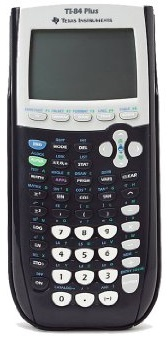
\includegraphics[height=0.3\textheight]{../../Common/figures/TI84.jpg}}
\end{picture}
\end{frame}

\begin{frame}
\frametitle{Wat is de cursus?}
\framesubtitle{Opzet}

\begin{itemize} %TODO: Variable over time
  \item !?!?? Wekelijks op Maandagavond 19:00-21:00.
  \pause
  \item Van DD/MM/YY tot DD/MM/YY, in totaal 5 keer.
  \pause
  \item Les bestaat uit beetje uitleg, en veel zelf proberen.
  \pause
  \item Je krijgt opdrachten mee naar huis om zelf te oefenen.
\end{itemize}

\end{frame}

\begin{frame}
\frametitle{Notatie op deze slides}

Op deze slides zullen we drie verschillende lettertypen vinden.
Het huidige lettertype is normale tekst.

\pause
\tifonttxt{Dit lettertype wordt gebruikt om tekst van je rekenmachine te laten zien.} \inlineticalc{7 \> A: A \! 6}

\pause
Tekens als \tiPRGM, \tiGRAPH, \tiCOS,  \tiXTn\, en \tiENTER\, zijn fysieke knoppen van je rekenmachine.

\pause
En tekens als \tiLOne, \tiACOS, en \tiMATRIX\, zijn knoppen die je met \tiSecond\, kunt bereiken.
Deze knoppen staan boven andere knoppen. Bijvoorbeeld \tiTEST\, is gelijk aan \tiSecond\tiMATH.

\vspace{10 mm}
\visible<5->{
Nu\ldots Laten we beginnen! Rekenmachines bij de hand\ldots
}
\end{frame}


%% END %%
\section{Hoe open je een programma?}

\begin{frame}
\frametitle{\tifontbigtxt{NEW} \tiPRGM}

\visible<1-2>{\ticalcfig{\ticalcfigCircle{\ticalcfigCircleColThree}{0.615}}}
\visible<3>{\ticalcfig{\ticalcfigCircleEnter\ticalcfigCircleRight}}
\visible<4>{\ticalcfig{\ticalcfigCircleEnter \ticalcfigCircleAlpha\ticalcfigCircleSecond}}
\visible<5>{\ticalcfig{\ticalcfigCircleSecond\ticalcfigCircle{\ticalcfigCircleColTwo}{0.81}}}

We gaan ons eerste programma aanmaken.
\begin{itemize}
  \item Druk op \tiPRGM.
  \pause %1
  \item \lenitem{Tenzij je eerder een programma hebt gemaakt, zie je alleen \inlineticalc{EXEC \, EDIT \, NEW}.}
  \pause %2
  \item Blader met \tiRight\,naar \tifonttxt{NEW} en druk op \tiENTER.
  \pause %3
  \item \lenitem{Type een naam in. Een prgm naam is maximaal 8 karakters. Druk vervolgens op \tiENTER.}
	  \begin{ticalc}[3.25cm]
	  	PROGRAM\\
	  	NAME=MYPRGM01
	  \end{ticalc}
  
  Merk op dat je een \tiCursorAlpha-cursor hebt: \tiALOCK\,is geactiveerd.
  \pause %4
  \item Sluit het programma nu met \tiQUIT.
\end{itemize}
\end{frame}

\begin{frame}
\frametitle{\tifontbigtxt{EDIT} \tiPRGM}

\visible<1-2>{\ticalcfig{\ticalcfigCircle{\ticalcfigCircleColThree}{0.615}}}
\visible<3>{\ticalcfig{\ticalcfigCircleRight}}
\visible<4>{\ticalcfig{\ticalcfigCircleDown\ticalcfigCircleEnter}}
\visible<5>{\ticalcfig{}}
\visible<6>{\ticalcfig{\ticalcfigCircleAlpha}}

Om het programma nu weer te openen, doe:
\begin{itemize}
  \item Druk op \tiPRGM.
  \pause %1
  \item \lenitem{Je ziet nu een lijst met alle programmas die je kunt uitvoeren.}
	  \begin{ticalc}[3.25cm]
	  	EXEC \, EDIT \, NEW
	  	1:MYPRGM01
	  \end{ticalc}
  \pause %2
  \item Blader met \tiRight\,naar \tifonttxt{EDIT}.
  \pause %3
  \item Hier zie je dezelfde lijst. Gebruik \tiDown\, om naar je programma te bladeren en druk op \tiENTER.
  \pause %4
  \item Als alternatief, kun je ook het nummer intoetsen wat voor je programma staat. Dit is een hotkey om je programma te openen.
  \pause %5
  		Ook kun je met \tiALPHA\, de eerste letter van je programmanaam intoetsen om snel je programma te vinden
  		(indien je later een grotere lijst met programmas hebt dan 1).
\end{itemize}
\end{frame}

\begin{frame}
\frametitle{Deleten/Archiveren van een \tiPRGM}
	TODO?
\end{frame}



%% END %%
% \section{Introduction}

\subsection[Introduction]{Introduction Masterclass GR-Advanced}

\begin{frame}
\frametitle{}
\framesubtitle{Subtitles are optional}

\begin{itemize}
  \item
  \item
\end{itemize}
\end{frame}

\begin{frame}
\frametitle{}

% You can create overlays
\begin{itemize}
  \item using the \texttt{pause} command:
  \begin{itemize}
    \item First item.
    \pause
    \item Second item.
  \end{itemize}
  \item using overlay specifications:
  \begin{itemize}
    \item<3-> First item.
    \item<4-> Second item.
  \end{itemize}
  \item using the general \texttt{uncover} command:
  \begin{itemize}
    \uncover<5->{\item First item.}
    \uncover<6->{\item Second item.}
  \end{itemize}
\end{itemize}
\end{frame}


%% END %%
% \section{Introduction}

\subsection[Introduction]{Introduction Masterclass GR-Advanced}

\begin{frame}
\frametitle{}
\framesubtitle{Subtitles are optional}

\begin{itemize}
  \item
  \item
\end{itemize}
\end{frame}

\begin{frame}
\frametitle{}

% You can create overlays
\begin{itemize}
  \item using the \texttt{pause} command:
  \begin{itemize}
    \item First item.
    \pause
    \item Second item.
  \end{itemize}
  \item using overlay specifications:
  \begin{itemize}
    \item<3-> First item.
    \item<4-> Second item.
  \end{itemize}
  \item using the general \texttt{uncover} command:
  \begin{itemize}
    \uncover<5->{\item First item.}
    \uncover<6->{\item Second item.}
  \end{itemize}
\end{itemize}
\end{frame}


%% END %%
% \section{Introduction}

\subsection[Introduction]{Introduction Masterclass GR-Advanced}

\begin{frame}
\frametitle{}
\framesubtitle{Subtitles are optional}

\begin{itemize}
  \item
  \item
\end{itemize}
\end{frame}

\begin{frame}
\frametitle{}

% You can create overlays
\begin{itemize}
  \item using the \texttt{pause} command:
  \begin{itemize}
    \item First item.
    \pause
    \item Second item.
  \end{itemize}
  \item using overlay specifications:
  \begin{itemize}
    \item<3-> First item.
    \item<4-> Second item.
  \end{itemize}
  \item using the general \texttt{uncover} command:
  \begin{itemize}
    \uncover<5->{\item First item.}
    \uncover<6->{\item Second item.}
  \end{itemize}
\end{itemize}
\end{frame}


%% END %%
% \section{Introduction}

\subsection[Introduction]{Introduction Masterclass GR-Advanced}

\begin{frame}
\frametitle{}
\framesubtitle{Subtitles are optional}

\begin{itemize}
  \item
  \item
\end{itemize}
\end{frame}

\begin{frame}
\frametitle{}

% You can create overlays
\begin{itemize}
  \item using the \texttt{pause} command:
  \begin{itemize}
    \item First item.
    \pause
    \item Second item.
  \end{itemize}
  \item using overlay specifications:
  \begin{itemize}
    \item<3-> First item.
    \item<4-> Second item.
  \end{itemize}
  \item using the general \texttt{uncover} command:
  \begin{itemize}
    \uncover<5->{\item First item.}
    \uncover<6->{\item Second item.}
  \end{itemize}
\end{itemize}
\end{frame}


%% END %%
% \section{Introduction}

\subsection[Introduction]{Introduction Masterclass GR-Advanced}

\begin{frame}
\frametitle{}
\framesubtitle{Subtitles are optional}

\begin{itemize}
  \item
  \item
\end{itemize}
\end{frame}

\begin{frame}
\frametitle{}

% You can create overlays
\begin{itemize}
  \item using the \texttt{pause} command:
  \begin{itemize}
    \item First item.
    \pause
    \item Second item.
  \end{itemize}
  \item using overlay specifications:
  \begin{itemize}
    \item<3-> First item.
    \item<4-> Second item.
  \end{itemize}
  \item using the general \texttt{uncover} command:
  \begin{itemize}
    \uncover<5->{\item First item.}
    \uncover<6->{\item Second item.}
  \end{itemize}
\end{itemize}
\end{frame}


%% END %%
% \section{Introduction}

\subsection[Introduction]{Introduction Masterclass GR-Advanced}

\begin{frame}
\frametitle{}
\framesubtitle{Subtitles are optional}

\begin{itemize}
  \item
  \item
\end{itemize}
\end{frame}

\begin{frame}
\frametitle{}

% You can create overlays
\begin{itemize}
  \item using the \texttt{pause} command:
  \begin{itemize}
    \item First item.
    \pause
    \item Second item.
  \end{itemize}
  \item using overlay specifications:
  \begin{itemize}
    \item<3-> First item.
    \item<4-> Second item.
  \end{itemize}
  \item using the general \texttt{uncover} command:
  \begin{itemize}
    \uncover<5->{\item First item.}
    \uncover<6->{\item Second item.}
  \end{itemize}
\end{itemize}
\end{frame}


%% END %%
% \section*{Summary}

\begin{frame}
\frametitle<presentation>{Summary}

\begin{itemize}
  \item The \alert{first main message} of your talk in one or two lines.
\end{itemize}

% The following outlook is optional.
\vskip0pt plus.5fill
\begin{itemize}
  \item Outlook
  \begin{itemize}
    \item Something you haven't solved.
    \item Something else you haven't solved.
  \end{itemize}
\end{itemize}
\end{frame}

%% END %%




\end{document}

%% END %%